\section{Introduction}
\label{sec:intro}
%\blfootnote{$^\spadesuit$ Contributed equally.}
Generative large language models (LLMs), such as ChatGPT~\cite{brown2020language} and GPT-4~\cite{openai2023gpt4}, have proven to be powerful in various application domains, including question answering, program synthesis, and task automation~\cite{zhang2019pretraining, liu2021makes}.
%%%
However, it is challenging to quickly and cheaply serve these LLMs due to their large volume of parameters, complex architectures, and high computational requirements.
For example, the largest GPT-3 architecture has 175 billion parameters, which requires more than eight NVIDIA 40GB A100 GPUs to store in half-precision floating points, and takes several seconds to serve a single inference request~\cite{brown2020language}.

An LLM generally takes as input a sequence of tokens, called {\em prompt}, and generates subsequent tokens one at a time, as shown in \Cref{fig:existing_approach}. 
%%%
The generation of each token in the sequence is conditioned on the input prompt and previously generated tokens and does not consider future tokens.
This approach is also called {\em autoregressive} decoding because each generated token is also used as input for generating future tokens.
This dependency between tokens is crucial for many NLP tasks that require preserving the order and context of the generated tokens, such as text completion~\cite{yu2022orca}.

% \begin{figure*}
%     \centering
%     \subfloat[Incremental decoding.]{
%     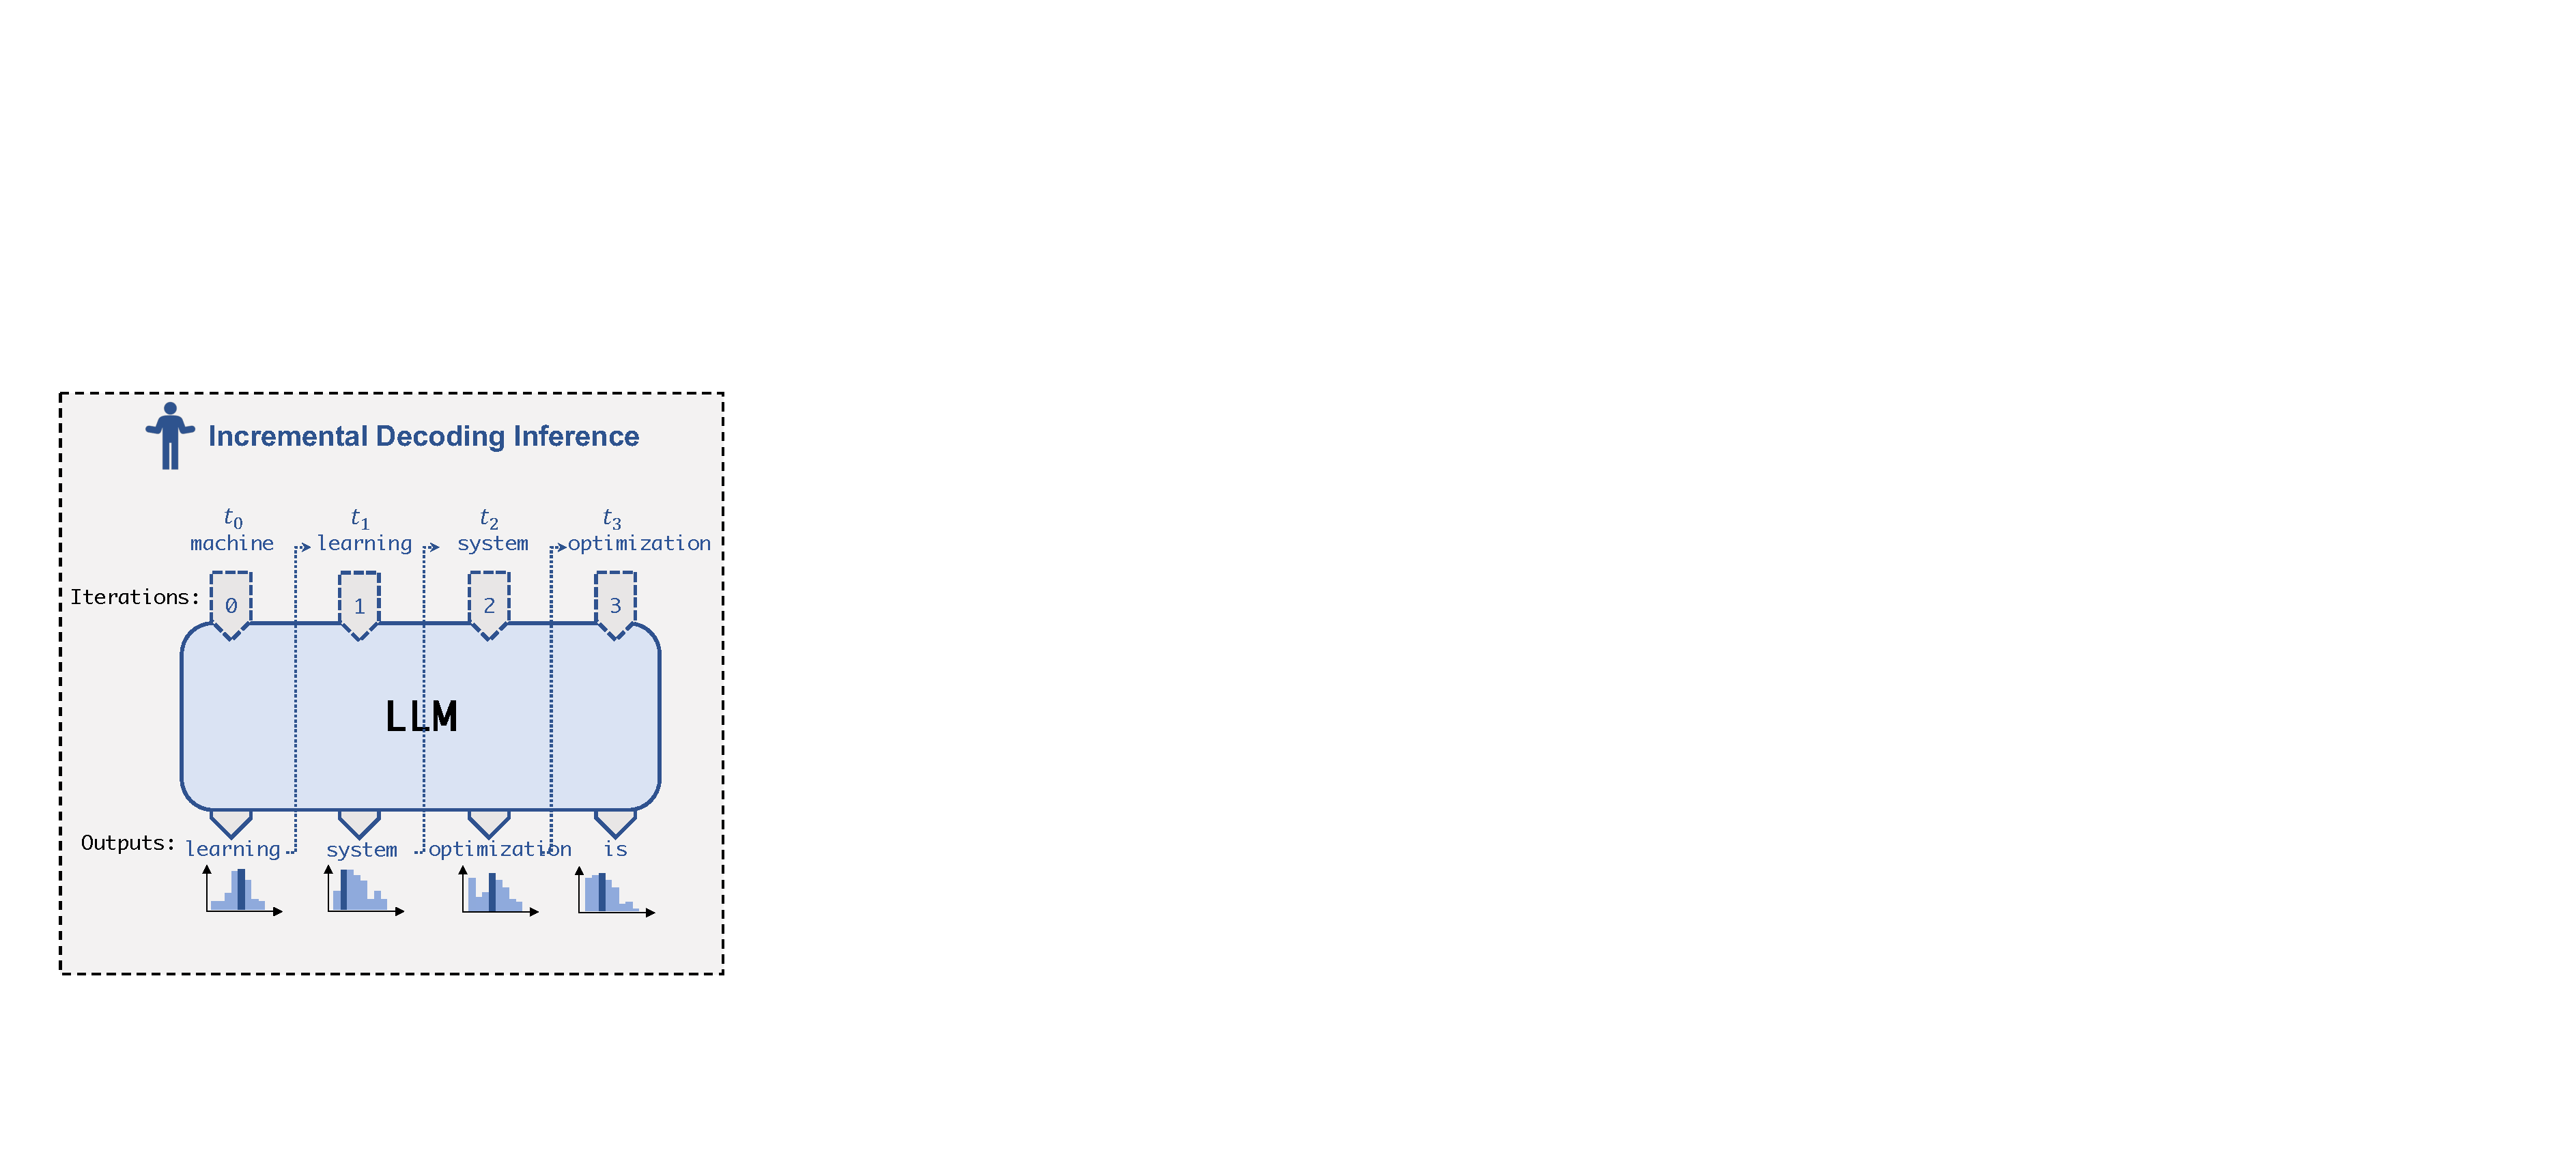
\includegraphics[scale=0.42]{rebuttal_figs/existing_overview6a3.pdf}
%     \label{fig:existing_approach}
%     }
%     \subfloat[\rev{Timeline Comparison.}]{
%     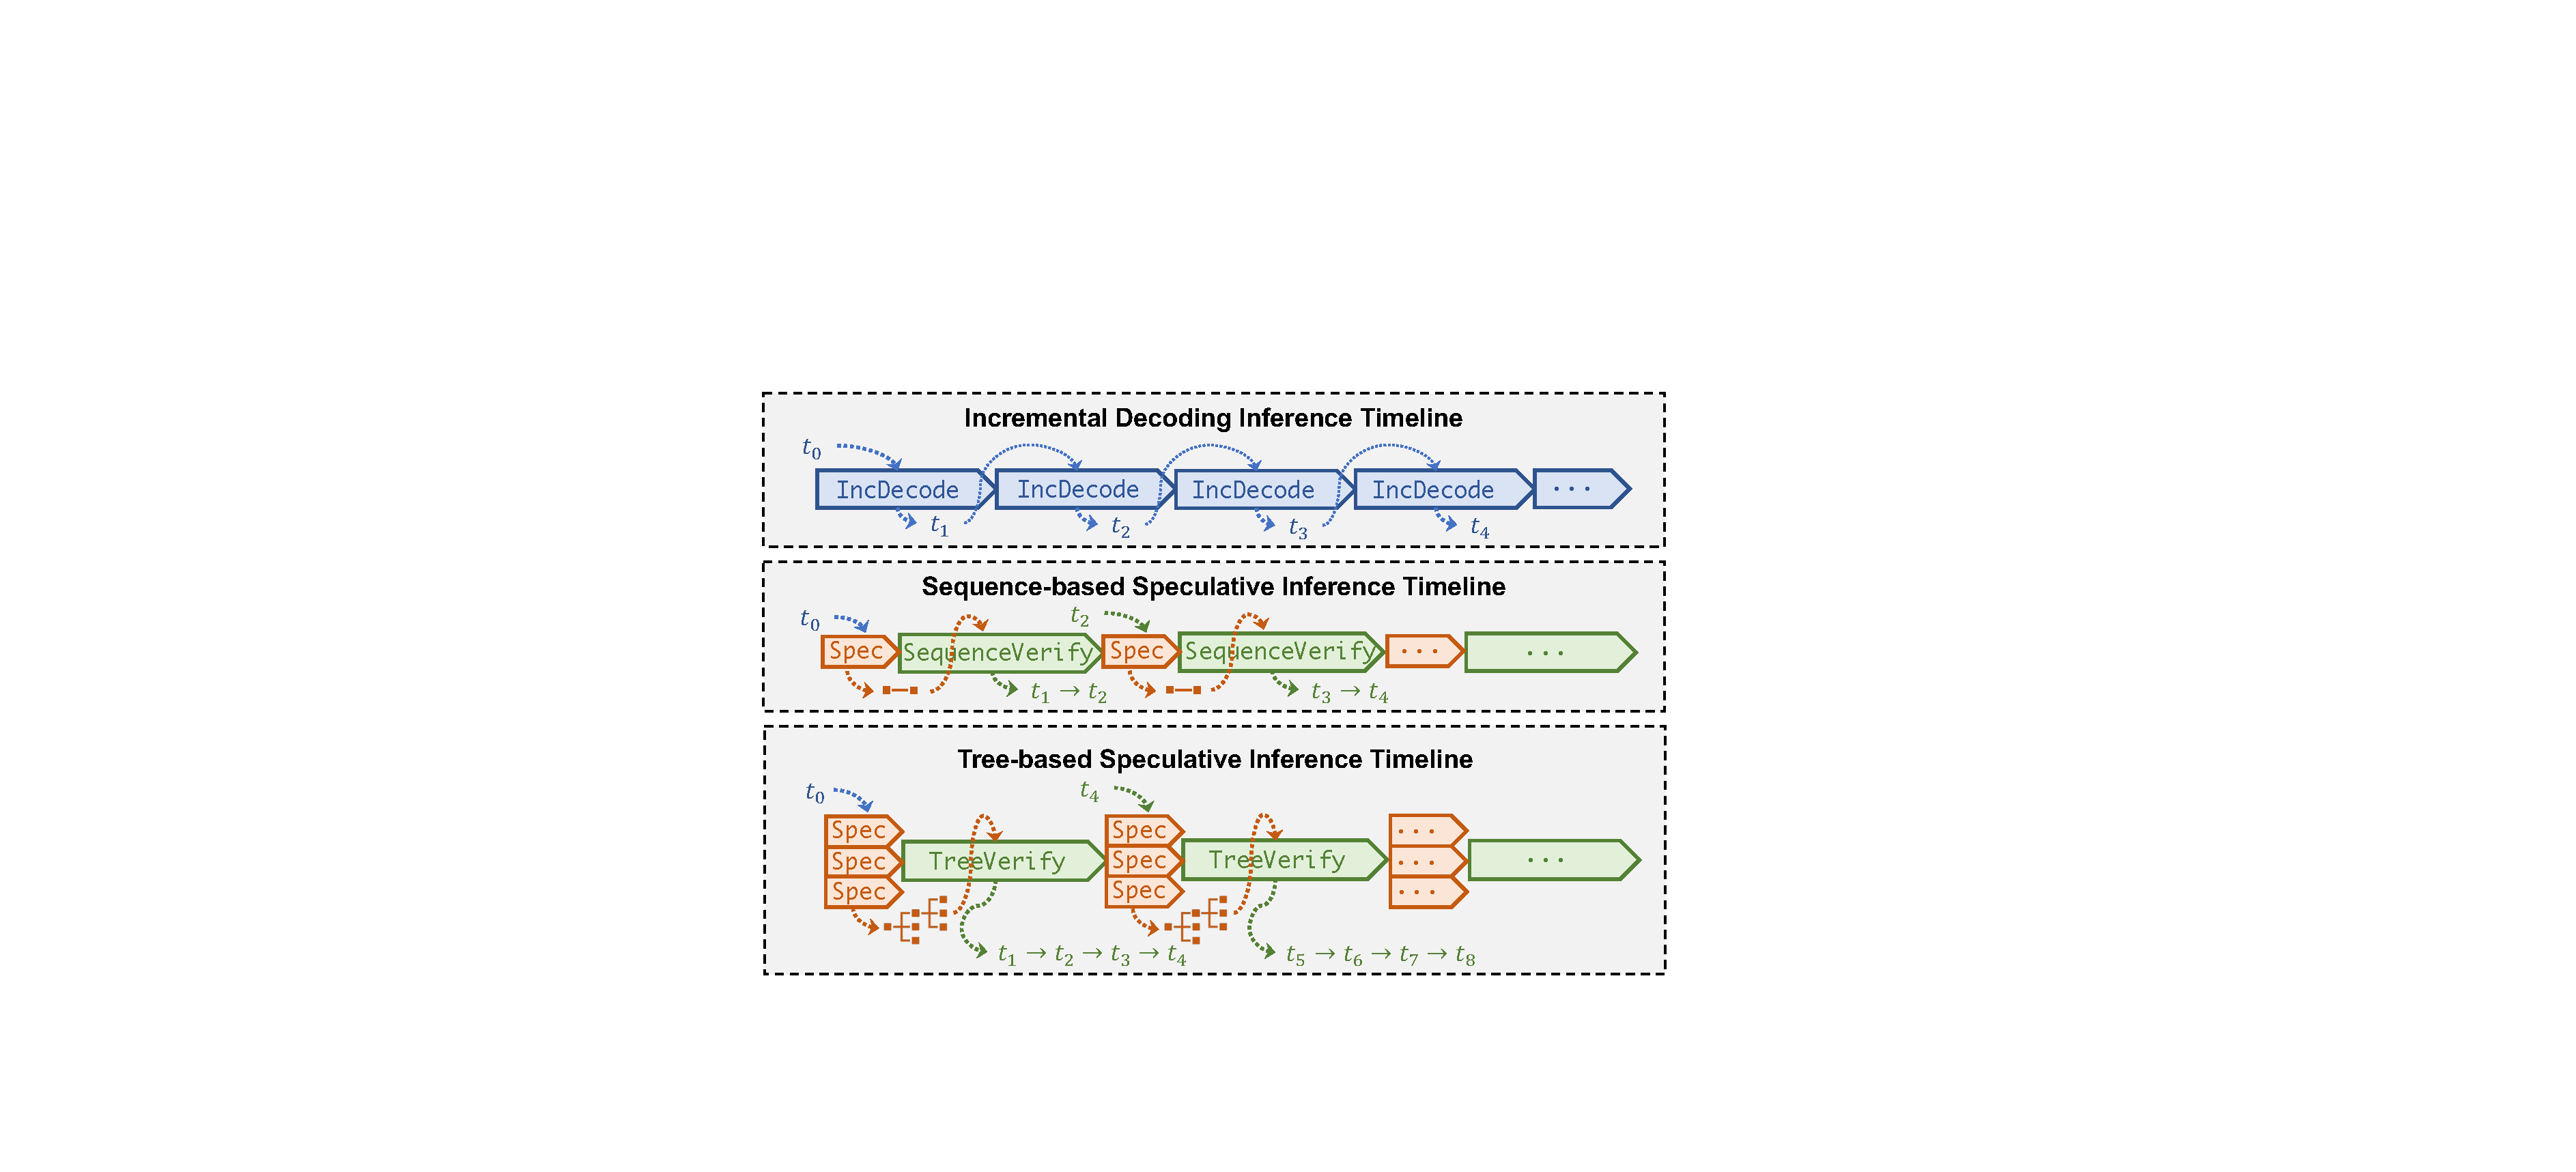
\includegraphics[scale=0.42]{rebuttal_figs/existing_overview6b5.pdf}
%     \label{fig:timeline}
%     }\\
%     \subfloat[\rev{Tree-based speculative inference and verification.}]{
%     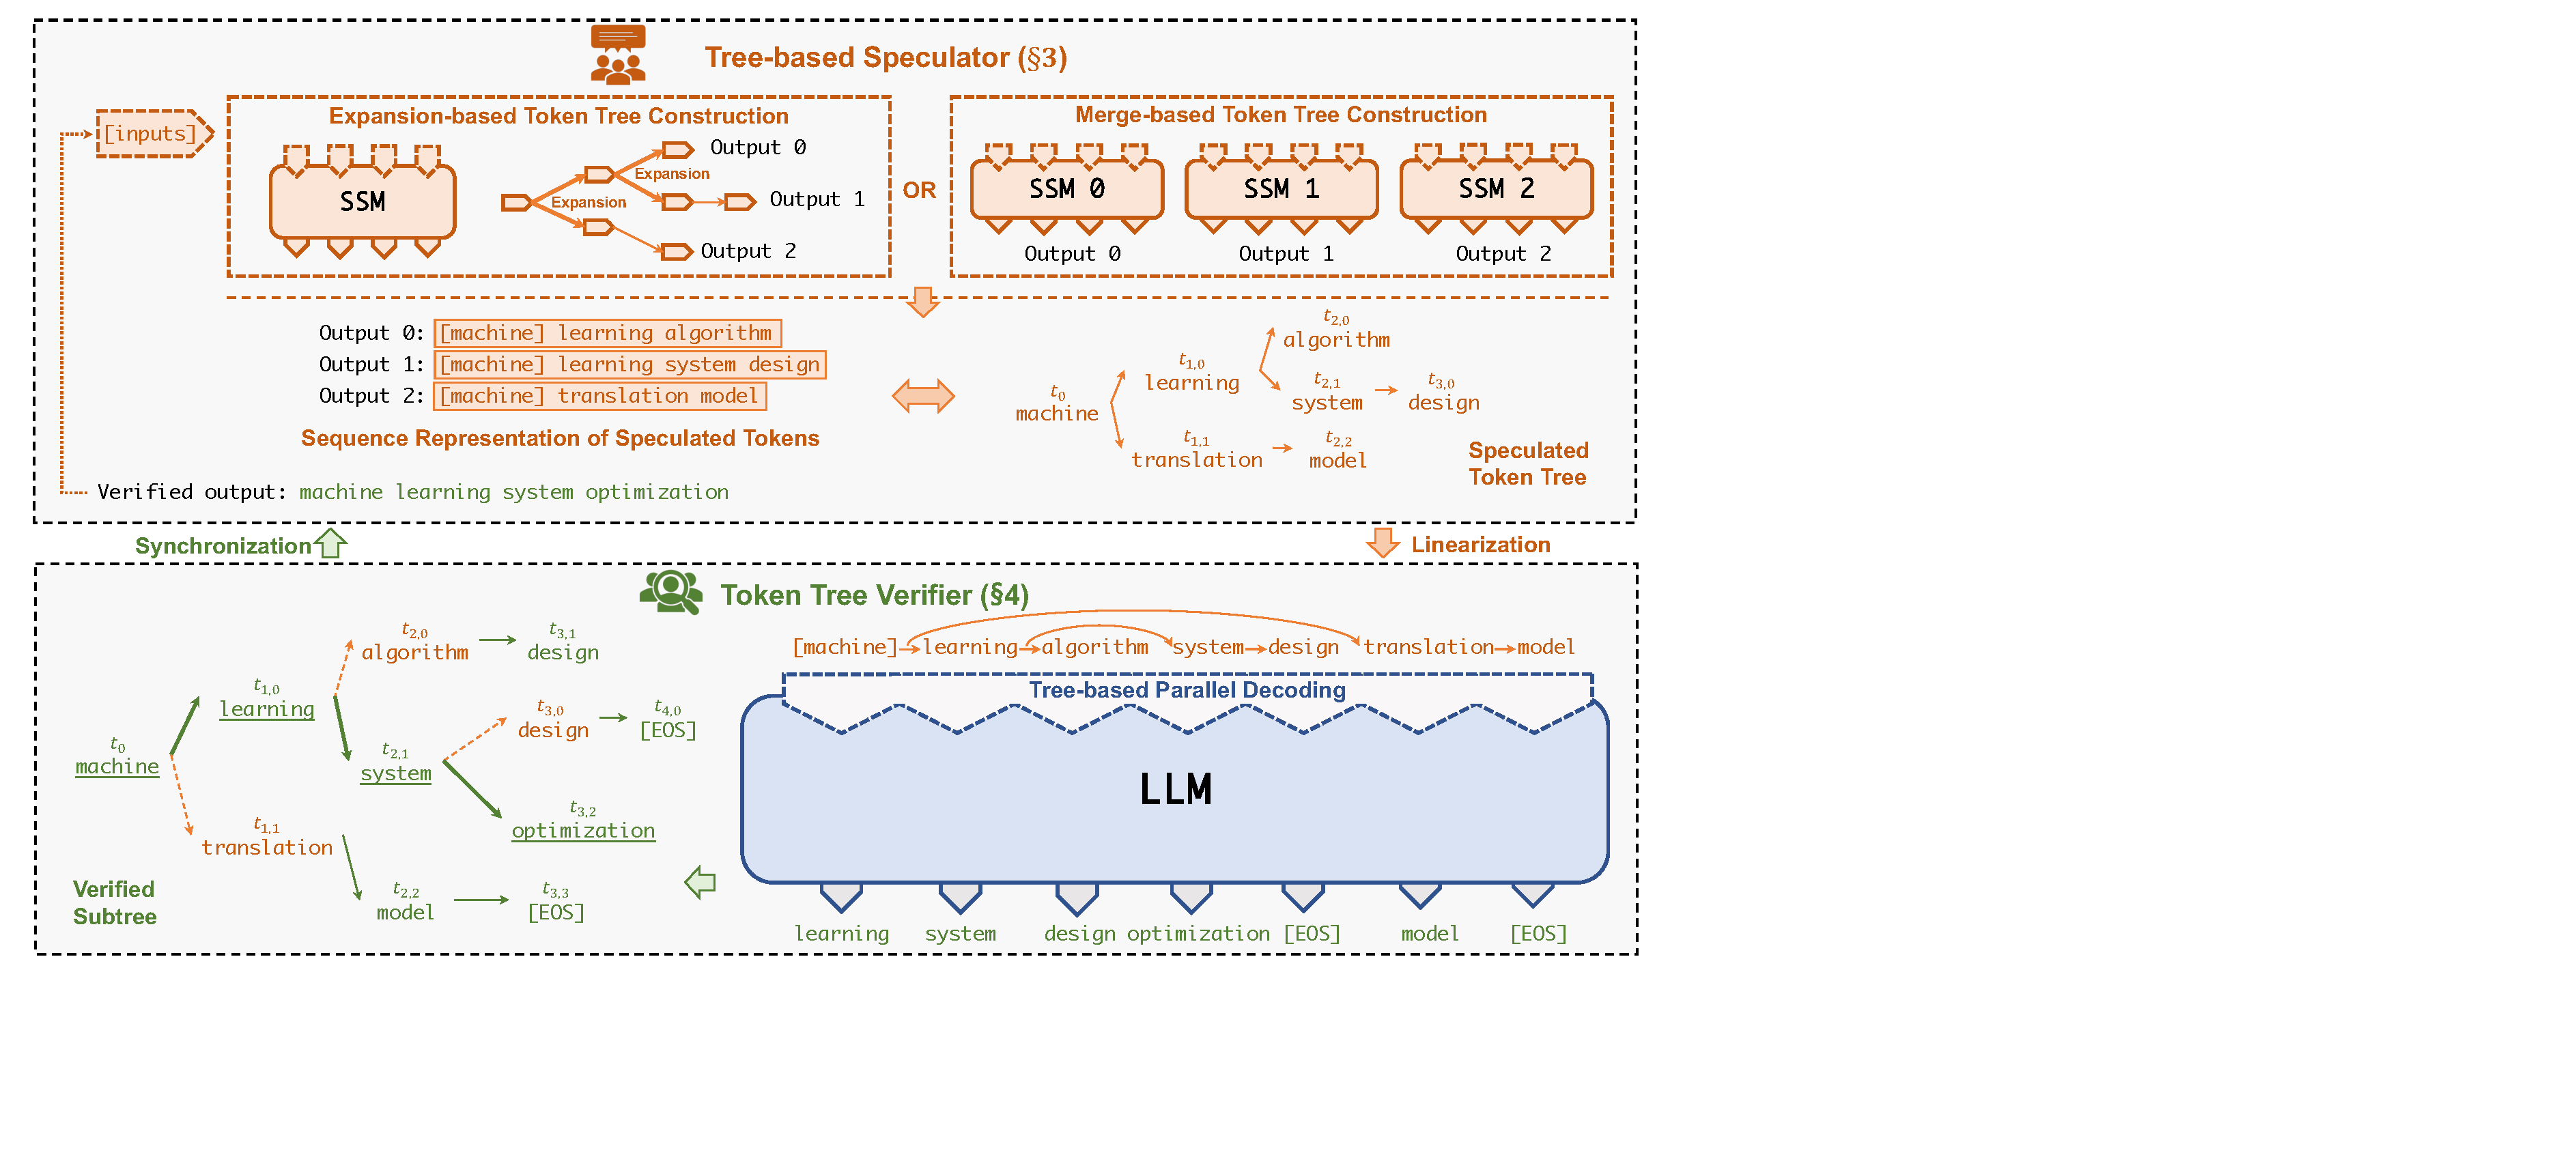
\includegraphics[scale=0.42]{rebuttal_figs/speculative_inference_overview8.pdf}
%     \label{fig:speculative_inference}
%     }
%     \caption{Comparing the incremental decoding approach used by existing LLM serving systems and the speculative inference and token tree verification approach used by \sys. \XM{Thinking to move figure (c) to page 3 or 4 as a separate overview figure}. \ZJ{I think that's a good idea. Can we also highlight the difference between existing sequence-based speculation and our proposed tree-based speculation?}}
%     \label{fig:specinfer_compared_to_incr_decoding}
% \end{figure*}

\begin{figure*}
    \centering
    \subfloat[Incremental decoding.]{
    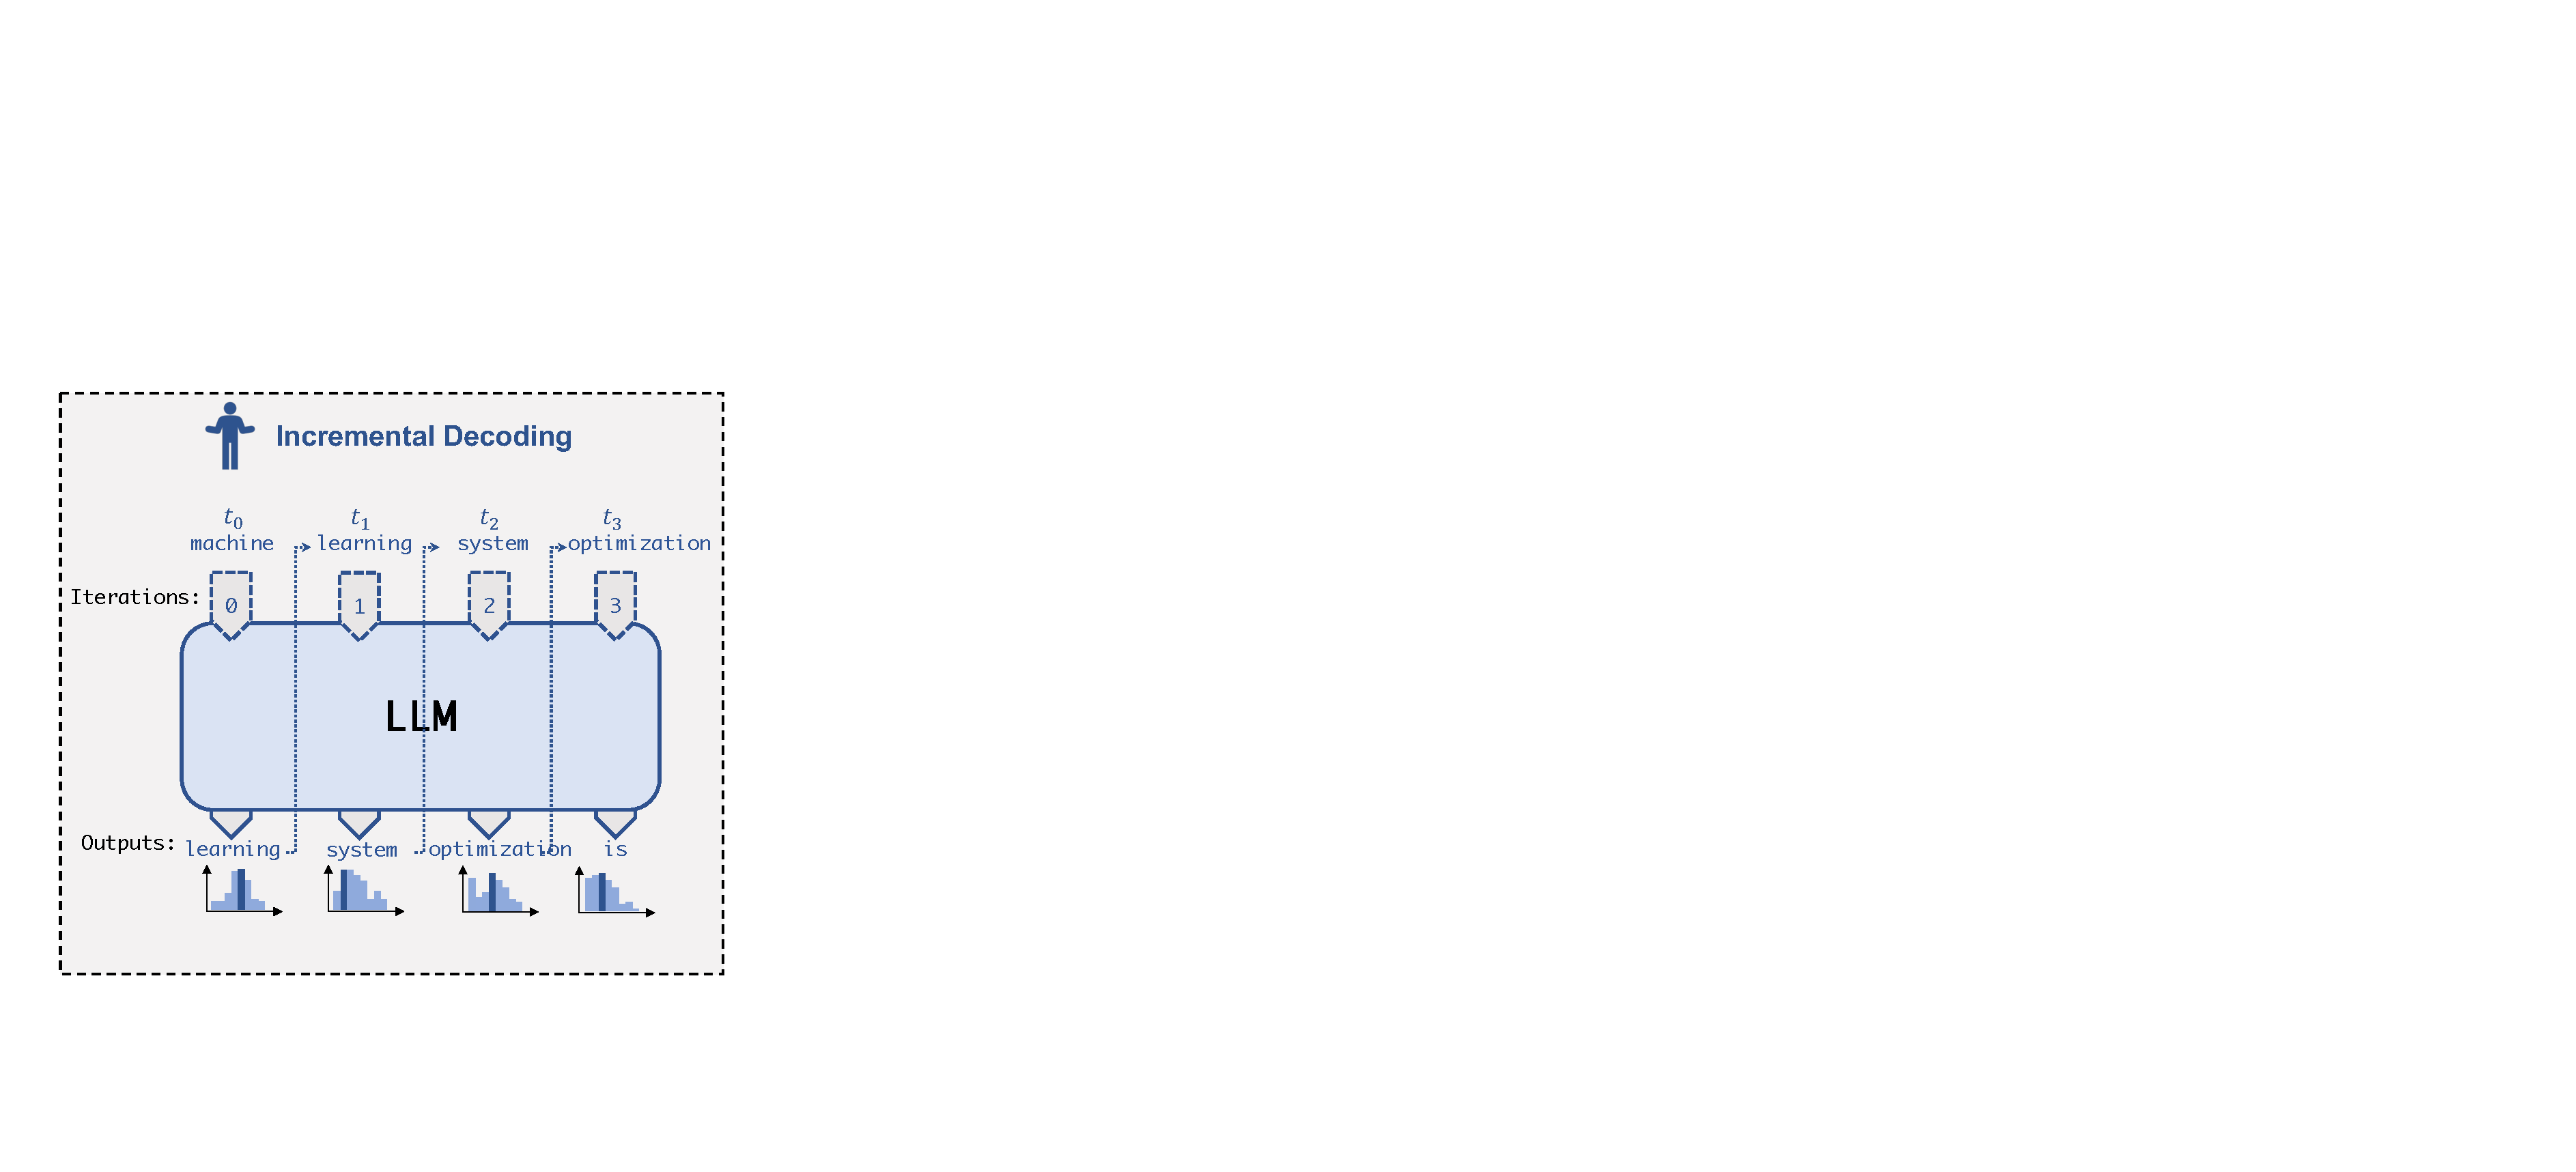
\includegraphics[scale=0.40]{rebuttal_figs/existing_overview6a4.pdf}
    \label{fig:existing_approach}
    }
    \subfloat[\rev{Timeline Comparison.}]{
    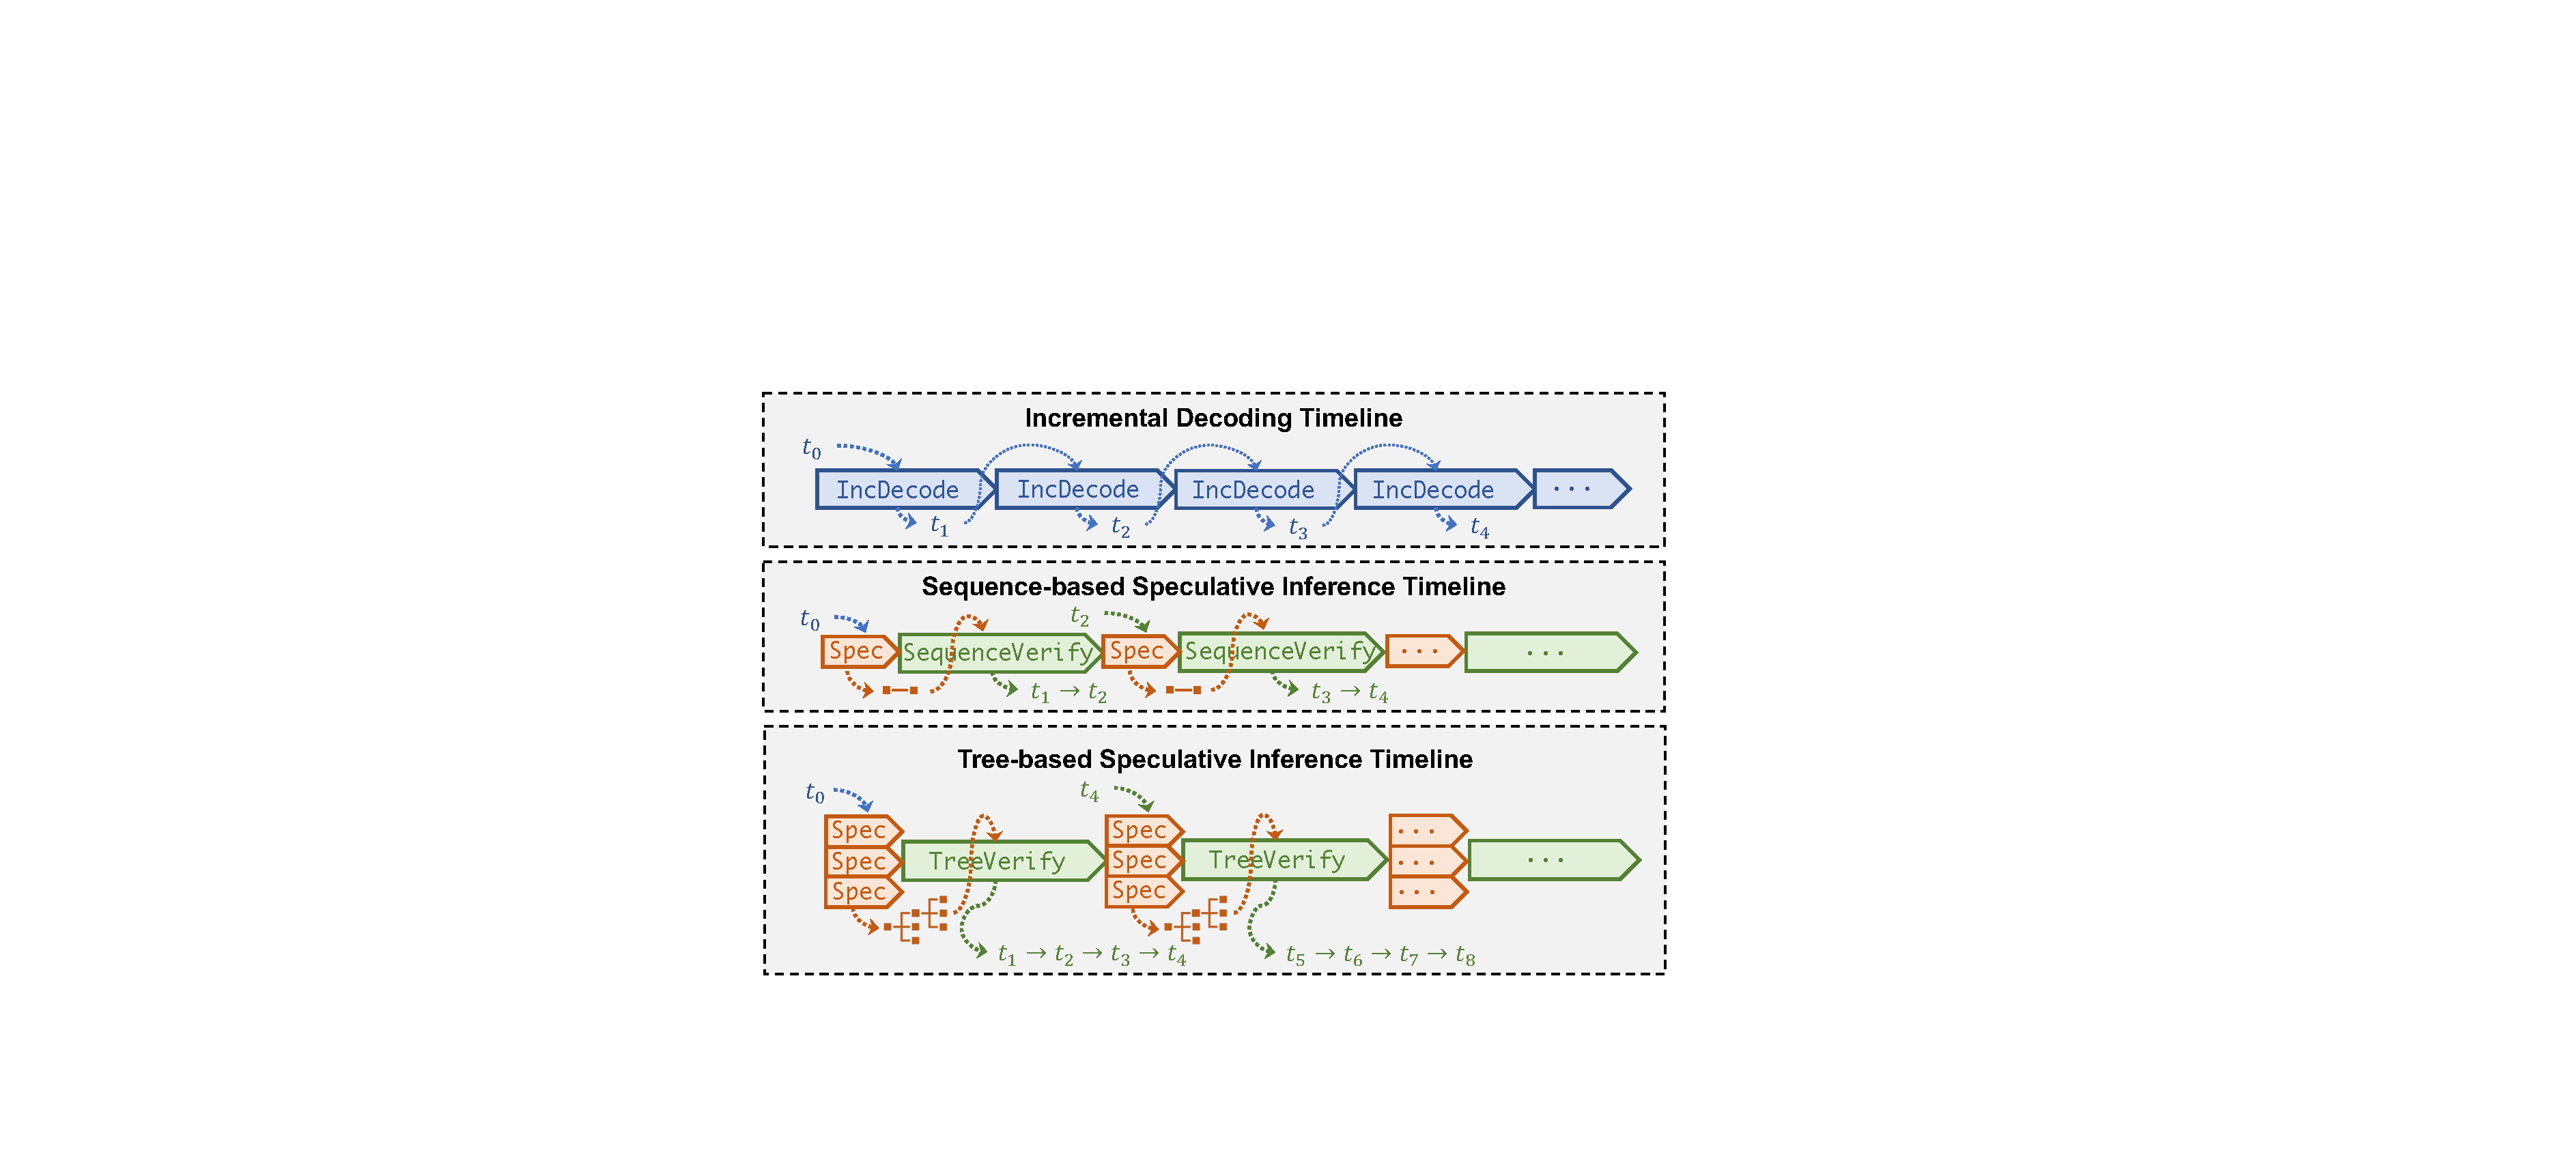
\includegraphics[scale=0.40]{rebuttal_figs/existing_overview6b6.pdf}
    \label{fig:timeline}
    }
    % \vspace{-4mm}
    \caption{\rev{Comparing the incremental decoding approach used by existing LLM serving systems, the sequence-based speculative inference approach, and the tree-based speculative inference approach used by \sys.}}
    \label{fig:specinfer_compared_to_incr_decoding}
\end{figure*}

Existing LLM systems generally use an {\em incremental decoding} approach to serving a request where the system computes the activations for all prompt tokens in a single step and then iteratively decodes {\em one} new token using the input prompt and all previously generated tokens~\cite{miao2023towards}. 
%%%
This approach respects data dependencies between tokens, but achieves suboptimal runtime performance and limited GPU utilization, since the degree of parallelism within each request is greatly limited in the incremental phase.
%%%
In addition, the attention mechanism of Transformer~\cite{vaswani2017attention} requires accessing the keys and values of all previous tokens to compute the attention output of a new token.
To avoid recomputing the keys and values for all preceding tokens, today's LLM systems use a caching mechanism to store their keys and values for reuse in future iterations.
For long-sequence generative tasks (e.g., GPT-4 supports up to 32K tokens in a request), caching keys and values introduces significant memory overhead, which prevents existing systems from serving a large number of requests in parallel due to the memory requirement of caching their keys and values.

\rev{Motivated by the idea of speculative execution in processor optimizations~\cite{gabbay1996speculative, smith1998study}, recent work introduces {\em sequence-based speculative inference}, which leverages a {\em small speculative model} (SSM) to generate a sequence of tokens and uses an LLM to examine their correctness in parallel~\cite{leviathan2022fast, xiaspeculative, stern2018blockwise, chen2023accelerating, gante2023assisted}.
%
These attempts only consider a token sequence generated by a single SSM for speculation, which cannot align well with an LLM due to the model capacity gap between them, since SSMs are generally orders of magnitude smaller than the LLM to maintain low memory and runtime overheads.
%Using a larger model can achieve better speculative performance but also introduces higher memory and runtime overheads.
}
%

%that iteratively decodes a {\em single} token using all previous tokens, as shown in \Cref{fig:existing_approach}. This approach achieves suboptimal performance and limited GPU utilization for serving LLMs since 

%This autoregressive inference approach achieves suboptimal performance and limited GPU utilization for two reasons. 
%%%
%First, unlike LLM training tasks where an ML system can simultaneously process {\em all} tokens of each training sample, a generative LLM serving system can only process {\em one} token at a time, which significantly limits the degree of parallelism within each request.
%Second, the attention mechanism of Transformer requires accessing the keys and values of all prompt tokens and previously generated tokens to compute a representation for the new token. To avoid recomputing the keys and values of all preceding tokens, {\em incremental decoding}~\cite{fiarseq} has been commonly used in modern LLM inference system to cache the keys and values for reuse in future iterations. 
%For long-sequence generative tasks, caching the keys and values introduces significant memory overhead, which prevents existing LLM inference system from serving a large number of requests in parallel due to caching keys and values.

This paper introduces \sys, a system that improves the end-to-end latency and computational efficiency of LLM serving with {\em tree-based speculative inference and verification}.
\Cref{fig:timeline} illustrates a comparison between existing incremental decoding, sequence-based speculative inference, and our tree-based speculative inference.
A key insight behind \sys is to simultaneously consider a diversity of speculation candidates (instead of just one as in existing approaches) to maximize speculative performance.
%construct a tree of speculated candidates by exploiting diversity with a single SSM and across multiple SSMs.
%combine multiple SSMs to collectively predict the LLM's outputs. \XM{TODO: update}
%
These candidates are organized as a {\em token tree}, whose nodes each represents a sequence of speculated tokens.
%
The correctness of {\em all} candidate token sequences is verified against the LLM in parallel, which allows \sys to significantly increase the number of generated tokens in an LLM decoding step. 
%combine various collectively boost-tuned small speculative models (SSMs) to jointly predict the LLM's output and use the LLM to verify {\em all} predictions, which allows \sys to opportunistically decode multiple tokens in an LLM decoding step, while existing incremental decoding approach only generates one token in each step.
%%%
%The idea of {\em speculative execution} has been widely deployed in a variety of optimization tasks in computer architecture and systems, including branch prediction in modern pipelined processors and value prediction for pre-fetching memory and files~\cite{gabbay1996speculative, smith1998study}.
\rev{Compared with sequence-based speculative inference, leveraging tree structures can significantly improve the success rate of verifying a token (e.g., from 52-57\% to 96-97\% for stochastic decoding as shown in \Cref{tab:acceptance-rate}).}
%
However, realizing this improvement requires addressing two unique challenges. Next, we elaborate on these challenges and the main ideas \sys uses to address them.

First, \sys must explore an extremely large search space of candidate token sequences to maximize speculative performance. While the idea of speculative execution has been widely deployed in a variety of optimization tasks in computer architecture and systems, including branch prediction in modern pipelined processors and value prediction for pre-fetching memory and files~\cite{gabbay1996speculative, smith1998study}, the search space considered by \sys is significantly larger due to two reasons:
%However, speculative inference requires exploring a significantly larger search space than prior speculative techniques due to two reasons:
(1) modern LLMs generally involve very large vocabularies, and (2) maximizing speculative performance requires predicting multiple future tokens (instead of just the next token). For example, all LLMs in the OPT model family consider 50,272 different possible tokens in their vocabulary, while \sys can correctly predict the next 4 tokens on average. Achieving this goal requires considering a search space of $50272^4\approx6\times 10^{18}$ different combinations of tokens. 
%Even with a set of effectively pruned speculations within the large search space, the second challenge is to verify the correctness of the speculations against the LLM efficiently.

\sys leverages existing distilled, quantized, and/or pruned variants of an LLM, which we call small speculative models (SSMs), to guide speculation. 
%
A key challenging of using SSMs for speculative inference is that the alignment between an SSM and an LLM is inherently bounded by the model capacity gap, since an SSM is generally 100-1000$\times$ smaller than an LLM.
%
\rev{Instead of using a single SSM for sequence-based speculation, \sys maximizes speculative performance by simultaneously considering a variety of token sequences organized in a tree structure for a given input prompt.
%
\Sys introduces an {\em expansion}- and a {\em merge}-based mechanism for constructing token trees by exploiting diversity within a single SSM and across multiple SSMs, respectively.}
%\Sys introduces {\em collective boost-tuning} to cooperatively fine-tune a set of SSMs by aligning their {\em aggregated} prediction with the LLM, and combines these boost-tuned SSMs to jointly predict the LLM's output. \XM{TODO: update}
%


A second challenge \Sys must address is verifying the speculated tokens. Many LLM applications perform {\em stochastic decoding}, which samples the next token from a probability distribution instead of deterministically generating a token. 
%%%
To preserve an LLM's generative performance, \Sys must guarantee that its tree-based speculative inference and verification mechanism generates the next token by following the {\em exact same} probability distribution as incremental decoding.
%%%
To achieve this goal, we propose {\em multi-step speculative sampling}, a new sampling approach for SSMs that guarantees equivalence while maximizing the number of speculated tokens that can be verified.
%%%
To minimize the token tree verification cost, \sys introduces a {\em tree-based parallel decoding} mechanism, {\em simultaneously} verifying all tokens of a token tree against the LLM's output in a {\em single} LLM decoding step.

\if 0
To this end, we introduce two key techniques to maximize \sys's speculative performance. 
%%%
For a given prefix as the input, \Sys uses multiple collectively {\em boost-tuned} small speculative models (SSMs) to jointly generate a token tree, whose nodes each represent a candidate token sequence.
%\XM{a candidate token or a candidate token sequence?}\ZJ{A token sequence. Does a candidate sequence of tokens work better here?}.
%%%
The correctness of {\em all} token sequences represented by a token tree is then verified against the LLM's original output in parallel using a novel {\em tree-based parallel} decoding algorithm.
This approach allows \Sys to opportunistically verify multiple tokens in a single decoding step as long as the speculated token tree overlaps with the LLM's output.
\fi 
%\Sys then uses an LLM as a {\em token tree verifier} that verifies whether a speculated token tree overlaps with the token sequence generated by the LLM using incremental decoding.
%%%
%\Sys is able to verify {\em all} sequences represented by a token tree in parallel and can opportunistically decode multiple tokens in a single step.

By leveraging tree-based speculative inference and verification, \Sys accelerates both distributed LLM inference across multiple GPUs and offloading-based LLM inference on one GPU.
Our evaluation shows that \Sys outperforms existing LLM serving systems by 1.5-2.8$\times$ for distributed LLM inference and by 2.6-3.5$\times$ for offloading-based LLM inference, while preserving the same generative accuracy.
%
%\rev{We will make \sys publicly available after the ASPLOS review period to facilitate future research.}

To summarize, we make the following contributions:
\begin{itemize}
    \item We present \sys, a tree-based speculative inference and verification system for LLM serving.
    \item To maximize speculative performance, we propose a merge- and an expansion-based method to construct token trees by exploiting diversity within and across SSMs, respectively.
    \item To minimize verification cost, we introduce a tree-based parallel decoding mechanism to simultaneously verify all tokens of a token tree.
    \item We evaluate \sys and show that it outperforms existing systems by up to 2.8$\times$ for distributed inference and by up to 3.5$\times$ for offloading-based inference.
\end{itemize}


\if 0
%%%
Compared to incremental decoding, \Sys's speculative inference and token tree verification introduce small computation and memory overheads for generating and verifying speculated token trees.
%%%
However, by maximizing the number of tokens that can be successfully verified in a single LLM decoding step, \Sys greatly reduces the end-to-end inference latency and improves the computational efficiency for serving generative LLMs.
%reduce memory accesses to the LLM's parameters whenever the overlap between the speculated token tree and the LLM's output is not empty.
%%%
%Since the performance of LLM inference on modern GPUs is largely limited by accessing GPU device memory, \Sys's approach can also reduce LLMs' end-to-end inference latency.
%%%
We evaluate \Sys on two LLM families (i.e., \llama~\cite{touvron2023llama} and OPT~\cite{zhang2022opt}) and five prompt datasets. 
%%%
Our evaluation shows that \Sys can reduce the number of LLM decoding steps by up to $4.4\times$ ($3.7\times$ on average) and reduce the end-to-end inference latency by up to 2.8$\times$.
\fi 

\if 0
\begin{figure}
    \centering
    \subfloat[Incremental decoding]{
    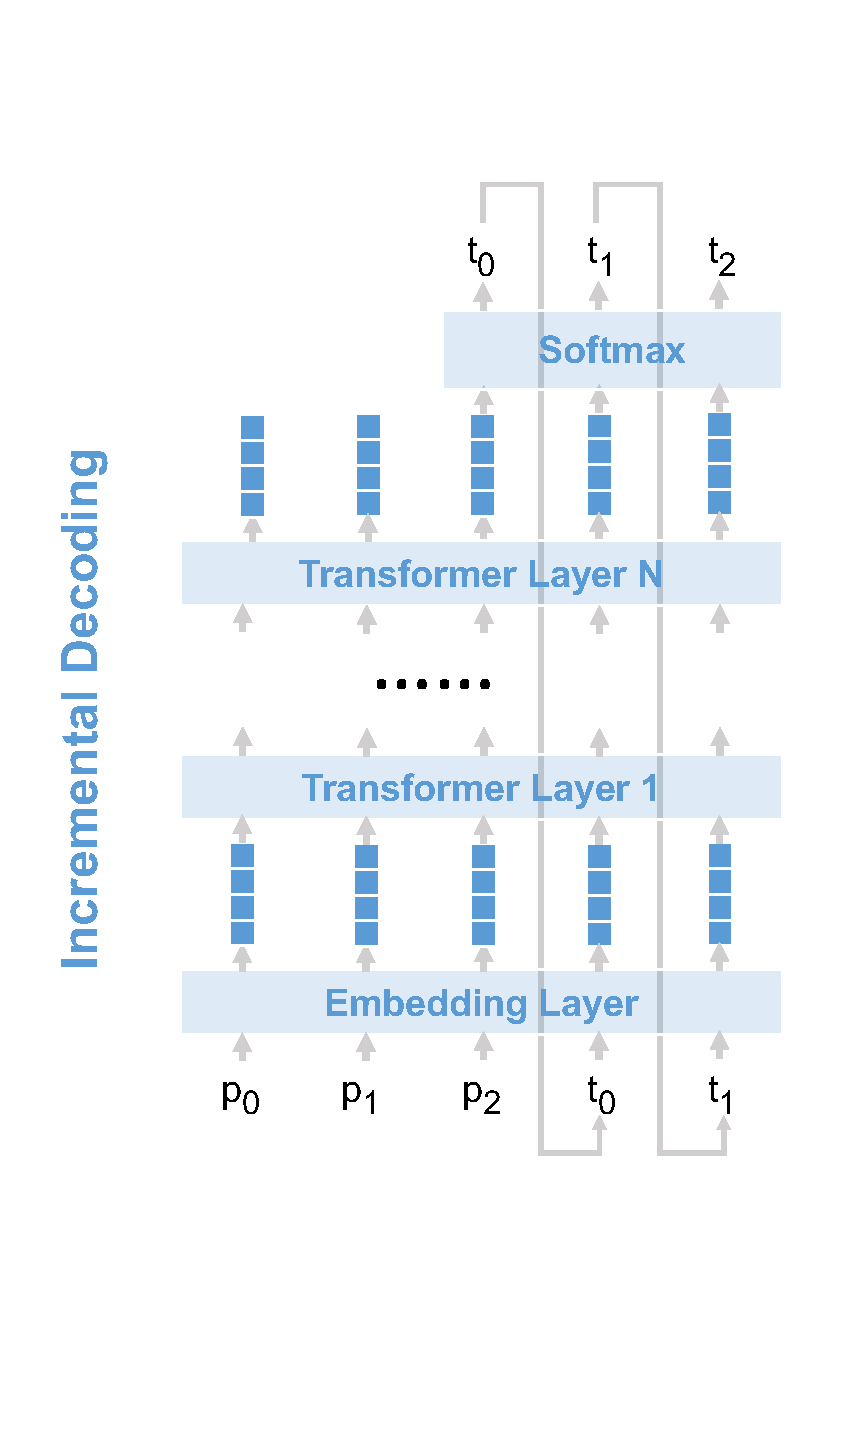
\includegraphics[scale=0.36]{figs/existing_overview.pdf}
    \label{fig:existing_approach}
    }
    \subfloat[Speculative inference with token tree verification.]{
    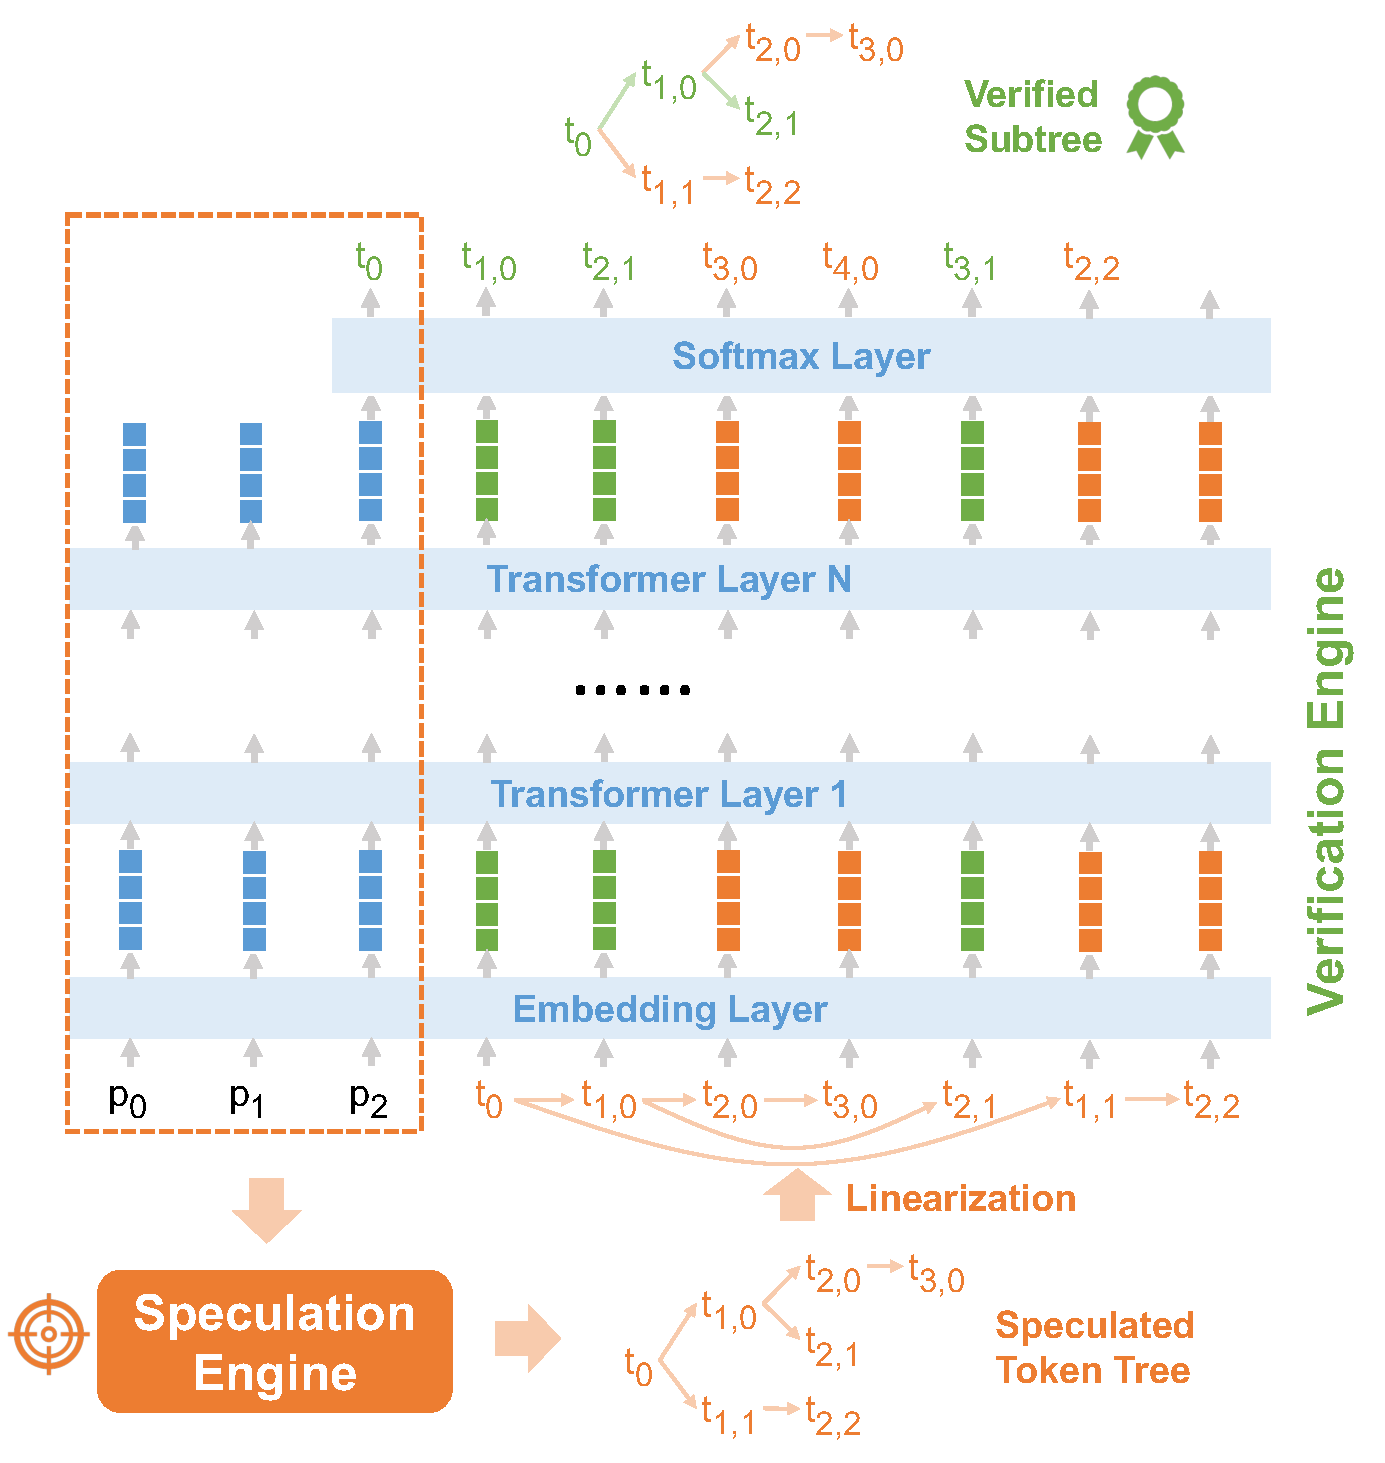
\includegraphics[scale=0.36]{figs/speculative_inference_overview.pdf}
    \label{fig:speculative_inference}
    }
    \caption{Comparing the incremental decoding approach used by existing LLM serving system and the speculative inference and token tree verification approach used by \sys.\XM{Do we want to highlight the difference between prompts and other tokens? Figure~\ref{fig:speculative_inference} might mislead the readers that the speculation engine can only accept prompts as inputs.} \ZJ{This is a great point. Any thoughts on how to improve this presentation? I am also thinking about using a real example to motivate our system.} \XM{(Done, To be replaced)}} 
\end{figure}
\fi
% \begin{figure}[t]
%     \centering
%     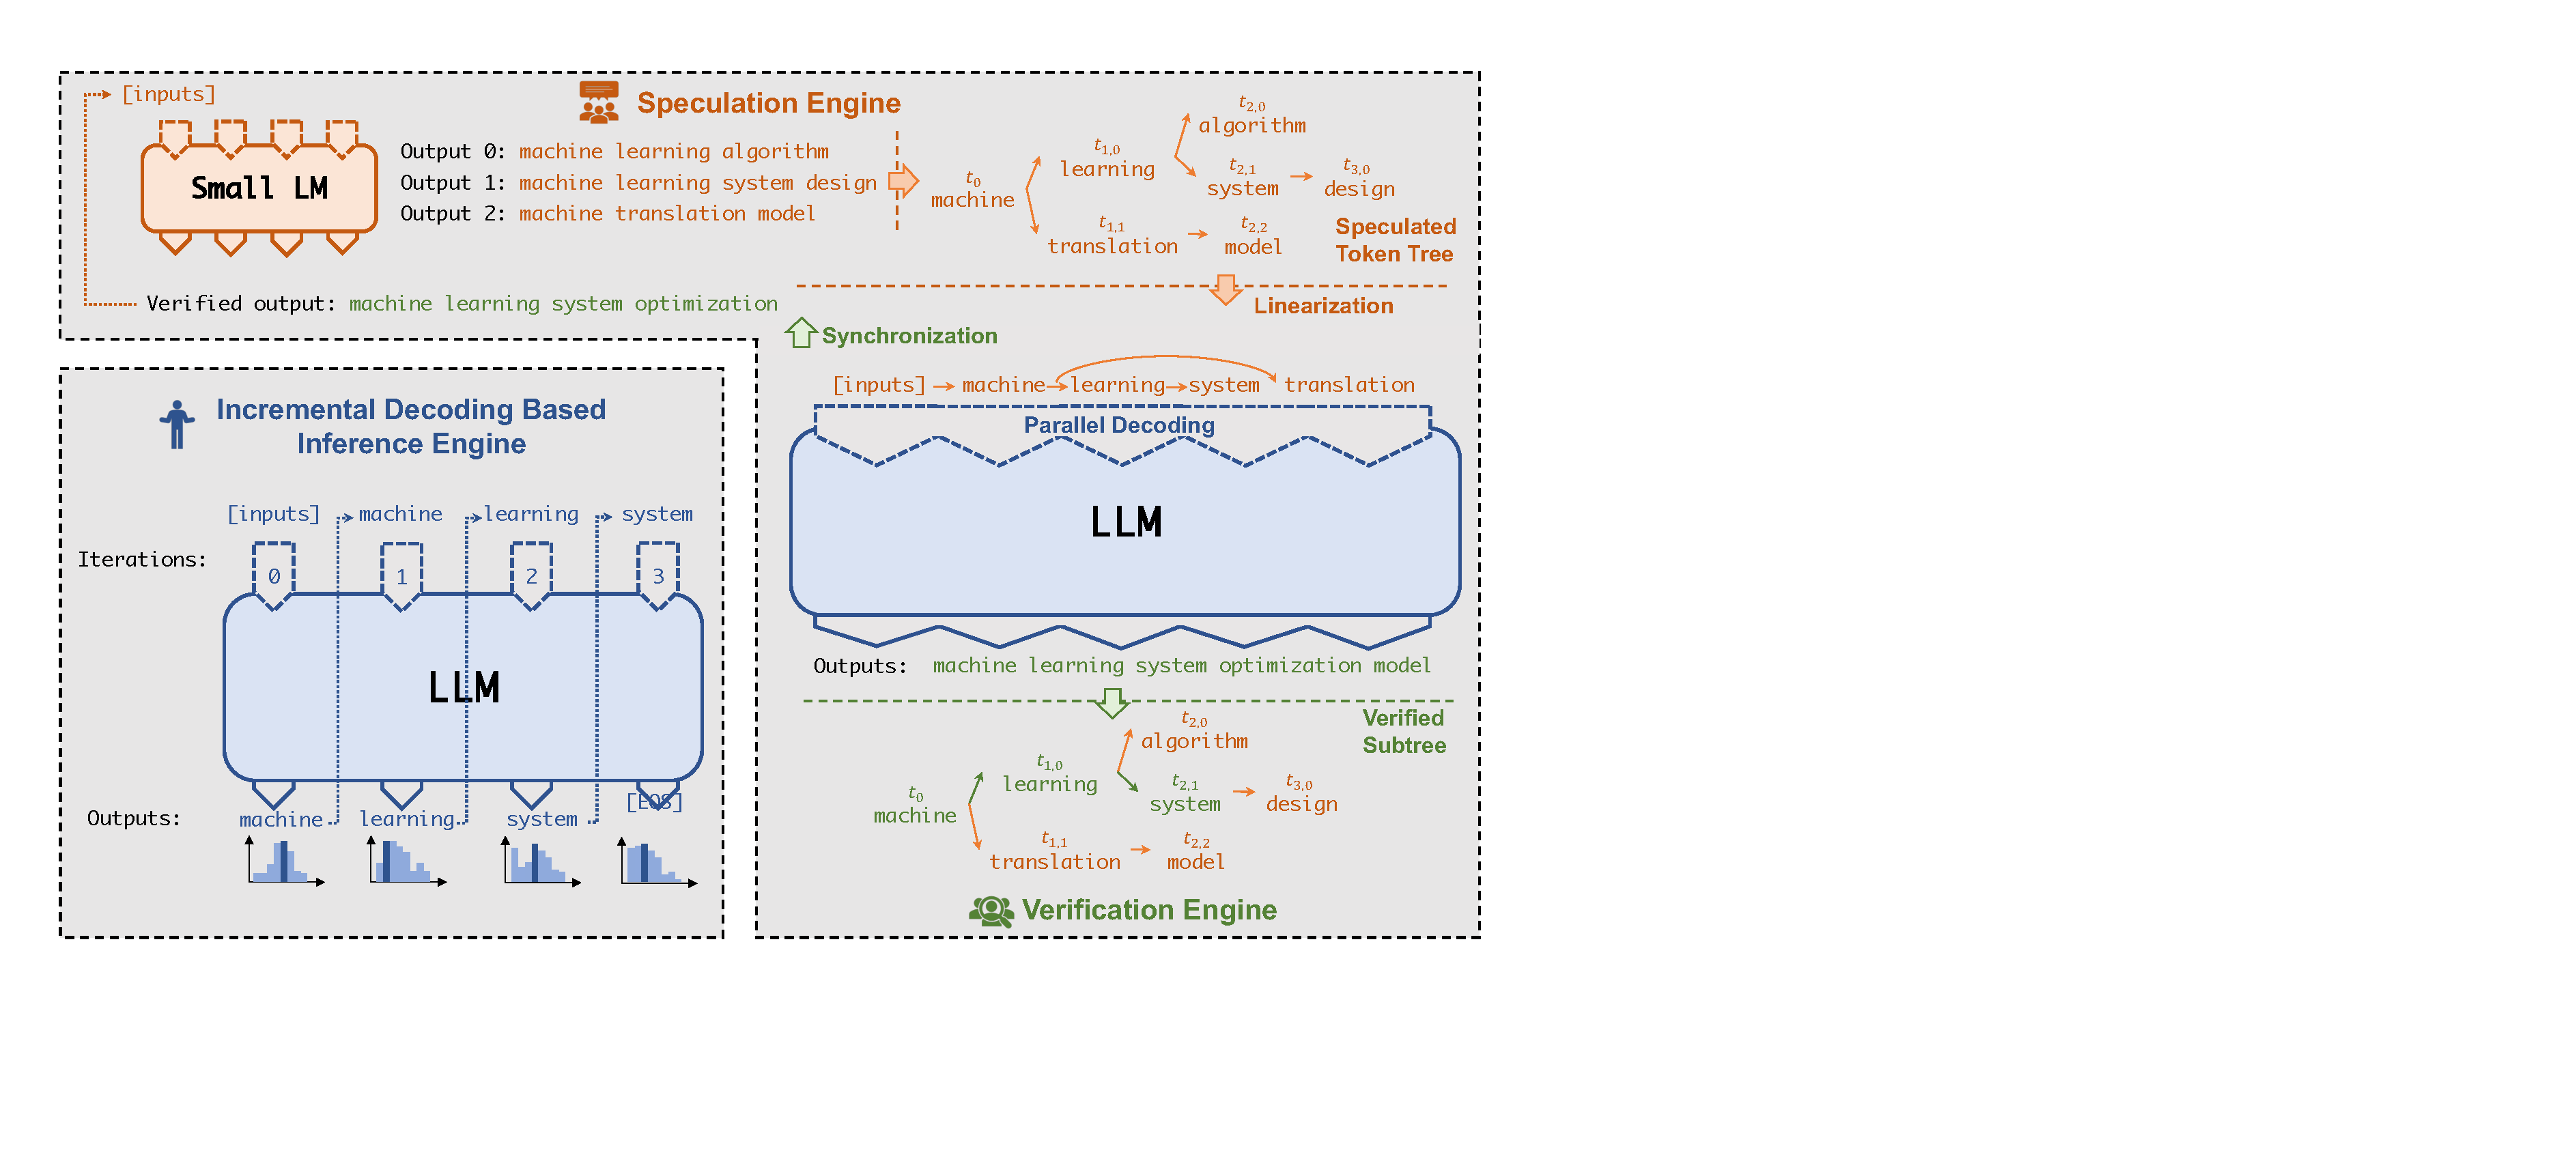
\includegraphics[width=1.0\textwidth]{figs/existing_overview4.pdf}
%     \label{fig:overview}
%     \caption{\XM{New figure}}
% \end{figure}
